% =====================================================================================
%  main_1.tex — Révision 1 de l'article de conférence IEEE (6 pages)
%  Révision du 27 octobre 2026, à partir de main.tex (version commentée par l'équipe).
%  Traçabilité : chaque modification porte une balise  % [Rxx]  (n° du commentaire de
%  l'équipe dans le PDF annoté) ou  % [Cxx]  (point de la lecture critique complémentaire).
%  Le contenu retiré du corps est déplacé dans le matériel supplémentaire
%  (supplementary_1.tex, sections S1–S6), cité dans le texte par « Supp. Sx ».
%  Options de mise en page (voir plus bas) : \figJtroistrue pour remplacer la vue 72 h
%  par la Fig. J3 (panneaux C et D) ; \titreoriginaltrue pour revenir à l'ancien titre.
% =====================================================================================
\documentclass[conference]{IEEEtran}
\IEEEoverridecommandlockouts
\usepackage{cite}
\usepackage[T1]{fontenc}
\usepackage[utf8]{inputenc}
\usepackage{textcomp}
\usepackage{amsmath,amssymb}
\usepackage{graphicx}\graphicspath{{figures/}}
\setkeys{Gin}{keepaspectratio}
\usepackage{booktabs,array}
\usepackage{adjustbox}
\usepackage{wasysym}
\usepackage{xcolor}
\usepackage[hidelinks]{hyperref}
% placement des flottants : autorise des pages plus riches en figures/tableaux
\renewcommand{\topfraction}{0.9}\renewcommand{\dbltopfraction}{0.9}\renewcommand{\bottomfraction}{0.8}
\renewcommand{\textfraction}{0.07}\renewcommand{\floatpagefraction}{0.85}\renewcommand{\dblfloatpagefraction}{0.85}
\setcounter{topnumber}{3}\setcounter{dbltopnumber}{3}\setcounter{totalnumber}{5}

\usepackage{newunicodechar}
\newunicodechar{●}{\CIRCLE}\newunicodechar{◐}{\LEFTcircle}\newunicodechar{○}{\Circle}
\newunicodechar{≈}{\ensuremath{\approx}}\newunicodechar{≤}{\ensuremath{\leq}}\newunicodechar{≥}{\ensuremath{\geq}}
\newunicodechar{→}{\ensuremath{\rightarrow}}\newunicodechar{−}{\ensuremath{-}}\newunicodechar{θ}{\ensuremath{\theta}}
\newunicodechar{×}{\ensuremath{\times}}

% ---------------- Options de la révision ----------------
\newif\iffigJtrois  \figJtroisfalse     % [R35][R36] false = Fig. 3 = vue 72 h (EN) ; true = Fig. J3 (C + D)
\newif\iftitreoriginal \titreoriginalfalse % [R15][R33] true = titre d'origine « Passive and Active »
% Raccourcis de notation [R32] : étiquettes en indice, exposants réservés aux puissances
\newcommand{\Penv}{P_{\mathrm{env}}}      % enveloppe dynamique (ancien E(k), libère E_d)
\newcommand{\PB}{P_{\mathrm{B}}}          % charge de référence S0
\newcommand{\Supp}[1]{Supp.~S#1}          % renvoi au matériel supplémentaire

\begin{document}
\iftitreoriginal
\title{Predictive Coordination of Passive and Active Thermal Flexibility in a Multi-Unit Residential Building to Relieve a Distribution Transformer during Winter Peaks}
\else
% [R15][R33] « passive » réservé au support de stockage ; les deux ressources sont pilotées activement
\title{Predictive Coordination of Building Thermal Mass and Electric Thermal Storage in a Multi-Unit Residential Building to Relieve a Distribution Transformer during Winter Peaks}
\fi

% [C1] Affiliations corrigées (Montréal, College) et numérotées dans l'ordre d'apparition
\author{%
\IEEEauthorblockN{%
Daniel Alain Anyouzo'o$^{1,*}$,
Nilson Henao$^{1}$,
David Toquica$^{1}$,
Kodjo Agbossou$^{1}$,\\
Follivi Kloutse$^{2}$,
Olivier Thierry Sosso$^{3}$,
Alejandro Parrado Duque$^{1}$}
\IEEEauthorblockA{%
$^{1}$Department of Electrical and Computer Engineering, Université du Québec à Trois-Rivières, QC G8Z 4M3, Canada\\
$^{2}$Hydro-Québec, Montréal, QC, Canada\\
$^{3}$Department of Electrical Engineering, Advanced Teachers' Training College for Technical Education, Douala, Cameroon\\
$^{*}$Corresponding author: daniel.alain.anyouzoo@uqtr.ca}%
}

\maketitle

% [R1][R2][R3][R4][R5] Résumé restructuré (contexte -> problème -> proposition -> résultats),
% sans sigles, sans « prohibitive », pourcentages rapportés à la référence.
\begin{abstract}
The simultaneous electrification of space heating and mobility makes heat-pump demand and unmanaged electric-vehicle charging coincide on winter evenings at the distribution transformers that supply multi-unit residential buildings. As an alternative to reinforcing these transformers, this paper proposes a two-layer predictive coordination that sequences two thermal storage resources by efficiency: the building envelope mass, preheated by heat pumps before the peak, and refractory-brick electric thermal storage units, which hold a lowered setpoint during the peak. An aggregator located at the transformer derives a scarcity signal from the transformer loading and aging rate and confines storage recharging under a dynamic power envelope that provably creates neither a new peak nor a rebound; each dwelling solves a convex predictive control problem based on a multizone thermal model identified from a digital twin. In a 72-hour case study of a 16-unit building supplied by a 50 kVA transformer, compared with conventional thermostats on the same days, the coordination reduces the evening peak by up to 19.3 \%, lowers the maximum hot-spot temperature from 86.4 to 62.4 °C and removes 99 \% of the discomfort at −17 °C, for a 4.5 \% increase in daily energy. When electric-vehicle charging alone exceeds the transformer capacity, thermal flexibility reaches a physical ceiling.
\end{abstract}
\begin{IEEEkeywords}
Distribution transformer, electric thermal storage, electric vehicles, model predictive control, multi-unit residential buildings, thermal flexibility, valley filling.
\end{IEEEkeywords}

% [R10] Nomenclature complète reclassée (Acronyms, Indices, Sets, Parameters, Variables)
% déplacée en Supp. S1 ; chaque sigle et symbole est défini à sa première occurrence [R17][R29].

\section{Introduction}

% [R6] référence ajoutée ; [R2][R7] définition de « uncoordinated » ; [R8] nuance sur la surcharge ;
% [R11] premature aging ; [R12] loading reserve ; [R13] gras retiré ; [R14] article du relecteur.
The simultaneous electrification of heating and transport increases and synchronizes residential demand \cite{NavarroEspinosa2016, Muratori2018}. In low-voltage networks, the joint deployment of heat pumps (HPs) and electric-vehicle (EV) chargers overloads distribution transformers \cite{NavarroEspinosa2016}. Uncoordinated charging, i.e., each EV charging at full power as soon as it is plugged in, without any signal from the utility or the building, concentrates in the early evening \cite{Muratori2018}. Although overloads represent a small fraction of the operating time of a distribution transformer, they concentrate on these coincident winter peaks, when insulation aging accelerates exponentially with the hot-spot temperature \cite{IEEEC5791_2025, IEC60076_7_2018}. Coordinated charging can mitigate this premature aging \cite{Hilshey2013}, and demand response combined with dynamic thermal rating (DTR) increases the transformer loading reserve and lifetime \cite{Daminov2021}. A poorly designed scheme may, however, worsen congestion: price-based scheduling of HPs and EVs synchronizes flexible loads to the point of exceeding the uncoordinated peak \cite{Hein2026}, and non-coordinated dynamic prices create rebound peaks by shifting demand \cite{ParradoDuque2027}. Relieving the transformer without reinforcement therefore calls on the building itself.

% [R15] Distinction support de stockage / stratégie : les deux ressources sont pilotées activement.
The thermal flexibility of buildings relies on two storage resources, both actively controlled:
\begin{itemize}
\item \emph{Structural storage}: the envelope mass shifts heating without dedicated equipment \cite{Reynders2013, LeDreau2016}; in Québec, a model predictive control (MPC) that preheats dwellings reduces the peak by about 30 \% compared with deadband control \cite{Vallianos2023}.
\item \emph{Dedicated storage}: refractory-brick electric thermal storage (ETS) units charge a massive core off-peak and release heat through controlled convection \cite{Devia2021}. Their combination with building mass has been studied for single-family houses \cite{EtedadiAliabadi2022}.
\end{itemize}

% [R16] répétition de « coordination » réduite
Exploiting both resources at building scale requires scheduling them jointly. Distributed home energy management systems (HEMS) based on the alternating direction method of multipliers (ADMM) enforce a common power limit \cite{Etedadi2023}. Multizone MPC has been applied to dwellings and small buildings \cite{Frahm2025, Hasrat2025}. For deferrable loads, valley filling is the reference for decentralized EV charging \cite{Gan2013}. Table~\ref{tab:I} positions these works against five criteria.

% [R33] en-tête de colonne harmonisé avec la nouvelle terminologie
\begin{table*}[tb]
\centering\footnotesize
\caption{Positioning (● addressed; ◐ partially; ○ not addressed; × not addressed, single dwelling; -- not applicable).}\label{tab:I}
\begin{tabular}{>{\raggedright\arraybackslash}p{\dimexpr0.171\linewidth-2\tabcolsep\relax}>{\raggedright\arraybackslash}p{\dimexpr0.143\linewidth-2\tabcolsep\relax}>{\raggedright\arraybackslash}p{\dimexpr0.169\linewidth-2\tabcolsep\relax}>{\raggedright\arraybackslash}p{\dimexpr0.150\linewidth-2\tabcolsep\relax}>{\raggedright\arraybackslash}p{\dimexpr0.182\linewidth-2\tabcolsep\relax}>{\raggedright\arraybackslash}p{\dimexpr0.174\linewidth-2\tabcolsep\relax}}
\toprule
\textbf{Work} & \textbf{Coupled multizone MUB} & \textbf{Envelope mass + ETS, coordinated} & \textbf{Transformer constraint} & \textbf{No-new-peak guarantee (trajectory)} & \textbf{Coordination} \\
\midrule
\cite{Etedadi2023} & × & ○ (envelope only) & fixed limit & ◐ (instantaneous) & iterative ADMM \\
\cite{EtedadiAliabadi2022} & × & ◐ (not coordinated) & ○ & ○ & distributed \\
\cite{Vallianos2023} & × & ◐ & ○ (price) & ○ & MPC \\
\cite{Frahm2025, Hasrat2025} & ● & ◐ & ○ & ○ & local / central MPC \\
\cite{Daminov2021} & -- & ○ & thermal (DTR) & ◐ & centralized \\
\cite{Gan2013} & -- & -- & ○ & ● (EV) & decentralized \\
\textbf{This work} & \textbf{●} & \textbf{●} & \textbf{fixed limit + aging} & \textbf{● (Prop. 1)} & \textbf{hierarchical, non-iterative} \\
\bottomrule
\end{tabular}
\end{table*}

% [R17] MUB défini ; [R18] G1 actualisée (travaux 2025–2026) ; [R19] lacunes en liste ;
% [R20][C15] G4 reformulée côté demande ; [R21-24][R25] trois contributions courtes, majuscules.
Table~\ref{tab:I} reveals four gaps:
\begin{itemize}
\item \textbf{G1.} Recent multizone models of multi-unit residential buildings (MUBs) represent each zone \cite{Frahm2025, Hasrat2025, Bisogno2026}, but inter-unit couplings are rarely identified in a verifiable way.
\item \textbf{G2.} Envelope mass (charged by HPs, COP ≈ 3) and ETS (COP = 1) are rarely \emph{ordered} by efficiency at multi-dwelling scale.
\item \textbf{G3.} Storage recharging is left to local optimizers: existing schemes guarantee an instantaneous limit, not the absence of a new peak or rebound over the trajectory \cite{Hein2026}.
\item \textbf{G4.} Although utilities routinely apply thermal loading guides and DTR \cite{IEEEC5791_2025, Daminov2021}, the signal sent to dwellings is rarely derived from the transformer thermal state.
\end{itemize}
The contributions of this paper are threefold:
\begin{enumerate}
\item A coupled multizone dwelling--storage model of an MUB, identified from data with an explicit identifiability check of inter-unit couplings (G1).
\item A two-layer predictive coordination that sequences envelope preheating and storage discharge by efficiency, driven by a transformer-aware scarcity signal (G2, G4).
\item A recharge envelope that provably creates neither a new peak nor a rebound, and a quantified physical ceiling of thermal peak shaving (G3).
\end{enumerate}
Supplementary material (Supp.~S1--S6: nomenclature, detailed model, identification, proof, parameters, additional results) accompanies the paper.

% [R28] Section limitée aux modèles ; les indicateurs de performance sont en Section IV-C.
\section{Modeling}\label{sec:model}

% [R26][R27] « coordination » remplacé ; [R29] phrase d'introduction de section
The transformer model defines the grid-side constraint; the dwelling and storage model describes the available flexibility.

\subsection{Transformer Thermal Model}

% [R32] k -> t (indice de temps), étiquettes en indice : theta_TO,u (ultimate) ; exposants x, y (IEC) ;
% rapport des pertes R -> R_L ; [R31] norme nommée et citée.
We use the method of §7.3.8 of IEEE Std C57.91-2025 \cite{IEEEC5791_2025}, consistent with IEC 60076-7 \cite{IEC60076_7_2018}. With $K=S/S_n$ the load factor, constant over a time step $\Delta t$ indexed by $t$, the exact discrete solution reads:
\begin{equation}\label{eq:to}
\adjustbox{max width=\linewidth}{$\displaystyle \begin{aligned}\theta_{TO}(t{+}1)&=\theta_{TO,u}(t)+\big(\theta_{TO}(t)-\theta_{TO,u}(t)\big)e^{-\Delta t/\tau_{TO}},\\ \theta_{TO,u}&=\theta_a+\Delta\theta_{TO,R}\left[\frac{K^2R_L+1}{R_L+1}\right]^{x}\end{aligned}$}
\end{equation}
\begin{equation}\label{eq:hs}
\adjustbox{max width=\linewidth}{$\displaystyle \begin{aligned}\Delta\theta_{H}(t{+}1)&=\Delta\theta_{H,R}K^{2y}+\big(\Delta\theta_{H}(t)-\Delta\theta_{H,R}K^{2y}\big)e^{-\Delta t/\tau_{w}},\\ \theta_{HS}&=\theta_{TO}+\Delta\theta_H\end{aligned}$}
\end{equation}
where $\theta_a$, $\theta_{TO}$ and $\theta_{HS}$ are the ambient, top-oil and hot-spot temperatures, $\theta_{TO,u}$ the ultimate top-oil temperature, $R_L$ the ratio of load to no-load losses, $\Delta\theta_{TO,R}$ and $\Delta\theta_{H,R}$ the rated rises, $\tau_{TO}$ and $\tau_w$ the oil and winding time constants, and $x=y=0.8$ the exponents for ONAN (oil natural, air natural) cooling (Table~6 of IEEE Std C57.91-2025 \cite{IEEEC5791_2025}). This exact form is unconditionally stable. For thermally upgraded paper, the aging acceleration factor follows the Arrhenius law \cite{IEEEC5791_2025}:
\begin{equation}\label{eq:faa}
F_{AA}=\exp\!\Big(\frac{15\,000}{383.15}-\frac{15\,000}{\theta_{HS}+273.15}\Big).
\end{equation}

\subsection{Multizone Dwelling and Storage Model}

% [R30] Développement détaillé (anciennes Éq. 4–7) en Supp. S2 : on garde l'équilibre de l'air
% (qui porte les couplages inter-logements, cœur de G1) et le modèle final discret.
% [R34] Une seule figure de modèle (étage + ETS) ; l'ancienne Fig. 1 et la vue 3D BEopt sont en Supp. S2.
% [C3] Un symbole = un sens : logement voisin n' (et non j, réservé au pas d'horizon).
Each dwelling $n$ is described by its indoor air ($T_{i,n}$) and envelope ($T_{e,n}$) temperatures. It exchanges heat with the outdoor air ($T_{ext}$), the adjacent dwellings $n'\in\mathcal A_n$, the corridor of its floor ($T_{h,p}$) and its ETS, whose core ($T_{c,n}$) and insulated casing ($T_{s,n}$) form a 2R2C network (Fig.~\ref{fig:rc}) \cite{Bacher2011}. The indoor-air balance carries the inter-unit couplings:
\begin{equation}\label{eq:air}
\adjustbox{max width=\linewidth}{$\displaystyle \begin{aligned}C_{i,n}\dot T_{i,n}={}&\frac{T_{e,n}-T_{i,n}}{R_{i,n}}+\sum_{n'\in\mathcal A_n}\frac{T_{i,n'}-T_{i,n}}{R_{nn'}}+\frac{T_{h,p}-T_{i,n}}{R_{h,n}}\\&+\frac{T_{s,n}-T_{i,n}}{R_{s,n}}+\mathrm{COP}\,P_{h,n}+Q_{ETS,n}+Q_{int,n}\end{aligned}$}
\end{equation}
where $C$ and $R$ denote heat capacities (J/K) and thermal resistances (K/W), $P_{h,n}$ the HP electric power, $Q_{ETS,n}$ the heat released by the ETS and $Q_{int,n}$ the occupancy gains. The envelope and ETS nodes follow analogous balances (\Supp{2}). With state $x_n=[T_{c},T_{s},T_{i},T_{e}]^\top$, input $u_n=[P_{h},Q_{ETS},P_{ETS}]^\top$, where $P_{ETS}$ is the ETS charging power, and disturbances $d_n=[T_{ext},Q_{int},T_{h,p},T_{i,n'}]^\top$, the model is linear, $\dot x_n=Ax_n+Bu_n+Ed_n$. The discharge is a control input bounded at the current state, which preserves convexity \cite{Devia2021}:
\begin{equation}\label{eq:qets}
\begin{aligned}&0\le Q_{ETS,n}\le\min\Big\{Q_{ETS,\max},\frac{T_{c,n}-T_{i,n}}{R_{conv,\min}}\Big\},\\ &\mathrm{SOC}_n=\frac{T_{c,n}-T_{c,\min}}{T_{c,\max}-T_{c,\min}}\end{aligned}
\end{equation}
where SOC is the state of charge. The system is discretized exactly with a zero-order hold:
\begin{equation}\label{eq:zoh}
\begin{aligned}&x_n(t{+}1)=A_dx_n(t)+B_du_n(t)+E_dd_n(t),\\ &\begin{bmatrix}A_d&[B_d\ E_d]\\0&I\end{bmatrix}=\exp\!\Big(\begin{bmatrix}A&[B\ E]\\0&0\end{bmatrix}\Delta t\Big)\end{aligned}
\end{equation}

\begin{figure}[tb]
\centering
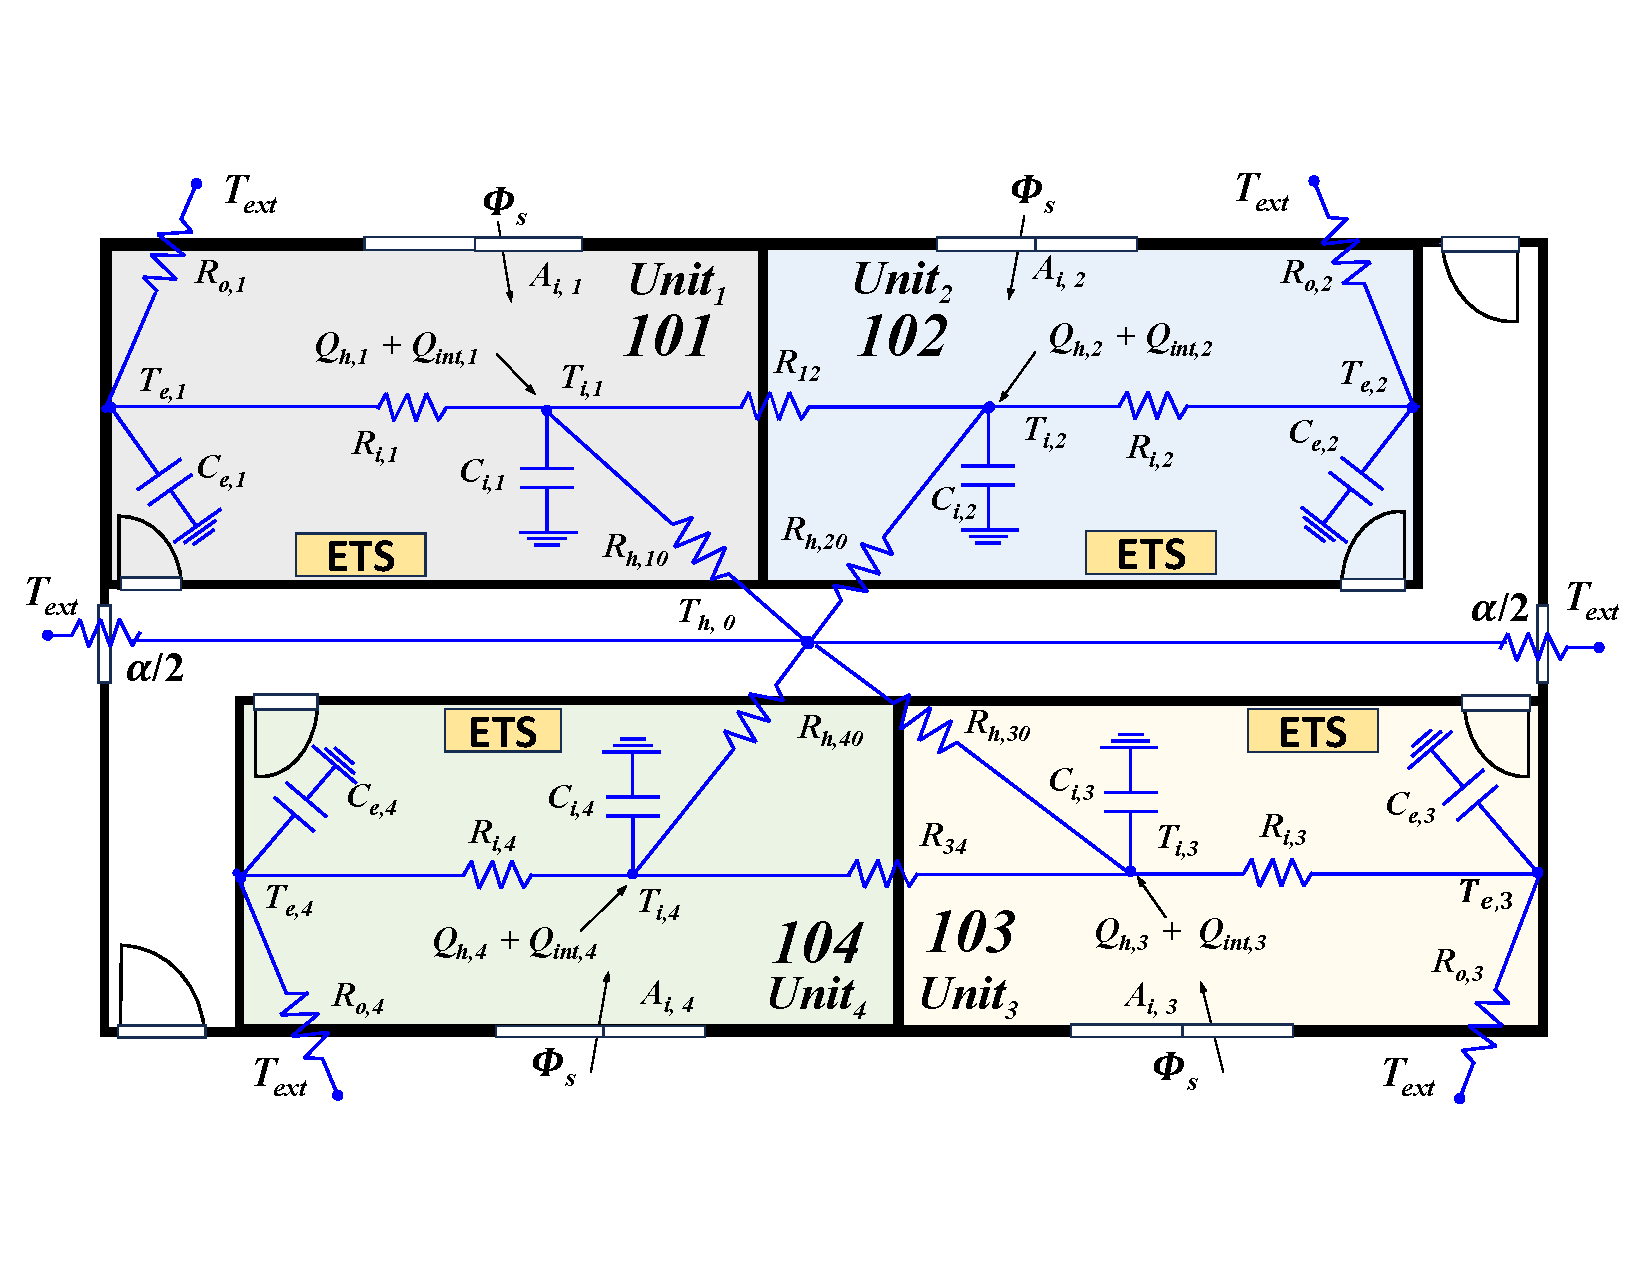
\includegraphics[width=0.9\linewidth]{fig3_palier.pdf}
\caption{Reduced 4R2C model of floor $p$ of the MUB (units 101--104, central corridor) with the 2R2C ETS of each unit: party-wall couplings $R_{12}$, $R_{34}$, corridor couplings $R_{h,n0}$ and solar apertures $A_{i,n}$.}
\label{fig:rc}
\end{figure}

\subsection{Identification of the Thermal Parameters}

% [R30][C4] Section condensée ; cadre EKF (ancienne Fig. 4), protocole, identifiabilité et
% Tableau II détaillés en Supp. S3. PRBS et NIS définis.
The parameters are identified from a BEopt 2.8.0 digital twin of the building \cite{BEopt28} (Trois-Rivières weather), with two one-month experiments per dwelling: a pseudo-random binary sequence (PRBS) setpoint excitation and a free-floating run. Estimation follows three steps \cite{Kristensen2004, Bacher2011}: an augmented-state extended Kalman filter (EKF) on $[T_i\ T_e\ \beta^\top]^\top$, with $\beta$ the log-parameters; an output-error refinement; and a maximum-likelihood tuning of the noise covariances. A Fisher-information analysis shows that couplings to neighbors and to the corridor are not excited when all units share the same setpoint, so they are fixed at their geometric values (\Supp{3}). On the test window, the 2-h (MPC horizon) prediction error is 0.78 °C and the normalized innovation squared (NIS) is 0.87--0.95, close to its ideal value of 1.

% [R26] « coordination » allégé
\section{Hierarchical Control Architecture}\label{sec:coord}

% [C2] Renvois de figures corrigés (\ref au lieu de numéros codés en dur).
The architecture has two layers (\Supp{2}): an \emph{aggregator} at the distribution transformer, which computes \emph{ex ante} the scarcity index, the phases of an automaton and the recharge envelope, then broadcasts the index and a power cap $c_n$; and a local HEMS-MPC agent that optimizes each dwelling. EV charging remains uncoordinated.

% [Pages] Figure d'architecture déplacée en Supp. S2 (fig4_arch.jpg).

\subsection{Reference Trajectory and Scarcity Index}

The aggregator first simulates the uncoordinated reference trajectory $\PB(t)=P_{nf}(t)+\sum_nP_{h,n,\mathrm B}(t)$, where $P_{nf}$ gathers the non-flexible base load and EV charging, and $P_{h,n,\mathrm B}$ is the power of proportional-integral-derivative (PID) controlled HPs tracking the same reference setpoint. This trajectory, assumed perfectly forecast, feeds \eqref{eq:to}--\eqref{eq:faa} and the dimensionless index:
\begin{equation}\label{eq:lambda}
\adjustbox{max width=\linewidth}{$\displaystyle \begin{aligned}\lambda(t)={}&w_L\min\Big\{1,e^{\kappa(u(t)-1)}\Big\}+w_T\min\Big\{1,\frac{F_{AA}(\theta_{HS,\mathrm B}(t))}{F_{AA}(120\,^\circ\mathrm{C})}\Big\},\\ &u=\PB/P_{lim},\quad P_{lim}=(1-K_s)S_n\mathrm{PF}\end{aligned}$}
\end{equation}
with $S_n$ the rated power, PF the power factor, $K_s$ a safety margin and $w_L+w_T=1$, so that $\lambda\in[0,1]$. The first term equals 1 at the safety limit and decays exponentially below it (steepness $\kappa$); the second is the normalized aging rate, equal to 1 when the predicted hot spot reaches 120 °C. A floor cost $\lambda_{pl}$ keeps off-peak energy from being free.

\subsection{Dynamic Setpoint}

% [C8] « 22:01 » remplacé par l'intervalle fermé équivalent au pas de 10 min ; T_j -> T_d (jour)
The reference setpoint applies the night setback recommended in Canada, a 2--3 °C reduction during sleep \cite{RNCan2024}: $T_{ref}(t)=T_d$ for $\mathrm{hr}(t)\in[06{:}00,22{:}00]$ and $T_d-\Delta T_n$ otherwise. The automaton then modulates the effective setpoint:
\begin{equation}\label{eq:tset}
T_{set}(t)=\begin{cases}T_{ref}+\Delta_{pre} & \text{preheating}\\ \min\{T_{ref},\,T_d-\Delta_{eff}\} & \text{congestion}\\ T_{ref} & \text{otherwise}\end{cases}
\end{equation}
and the comfort floor is $T_{min}=T_{set}-\delta$. Before the peak, the HP (COP ≈ 3) stores heat in the envelope mass by raising the setpoint by $\Delta_{pre}$. During the peak, the setpoint is lowered by $\Delta_{eff}$ within the comfort tolerance $\delta$: the free decay of $T_i$ first releases the envelope heat, then the ETS (COP = 1) holds the lowered setpoint. The $\min\{\cdot\}$ prevents the peak setback from adding to the night setback.

\subsection{Phase Automaton and Adaptive Curtailment}

Phases are determined \emph{ex ante} on the reference (Table~\ref{tab:phase}). The congestion set is $\mathcal C=\{t:\PB(t)\ge P_{lim}\}$, from which exceedances shorter than $\tau_{min}$ are removed (e.g., the morning reheat); these are handled by the envelope with $\Penv(t)=\max\{P_{lim},P_{nf}(t)\}$. During congestion, the HP is not switched off but limited to its share of the residual transformer margin, allocated in proportion to each dwelling's conductance $G_n$ to unheated zones:
\begin{equation}\label{eq:gamma}
\gamma_n=\frac{G_n}{\sum_lG_l},\qquad G_n=\frac{1}{R_{i,n}+R_{o,n}}+\frac{1}{R_{h,n}}
\end{equation}
where $R_{o,n}$ is the envelope--outdoor resistance. When $P_{nf}>P_{lim}$, the margin is zero and the coordinated load equals $P_{nf}$: the peak reduction is then bounded by the heating share of the reference peak, $\Delta P_{\max}/P_{\mathrm B,\max}\le P_{h,\mathrm B}(t^*)/\PB(t^*)$.

\begin{table*}[tb]
\centering\footnotesize
\caption{Phase automaton (evaluated at each horizon step $j$).}\label{tab:phase}
\begin{tabular}{>{\raggedright\arraybackslash}p{\dimexpr0.144\linewidth-2\tabcolsep\relax}>{\raggedright\arraybackslash}p{\dimexpr0.269\linewidth-2\tabcolsep\relax}>{\raggedright\arraybackslash}p{\dimexpr0.242\linewidth-2\tabcolsep\relax}>{\raggedright\arraybackslash}p{\dimexpr0.335\linewidth-2\tabcolsep\relax}}
\toprule
\textbf{Phase} & \textbf{Condition} & \textbf{Setpoint} & \textbf{Bounds imposed on agent $n$} \\
\midrule
0 Normal & none of the others & $T_{ref}$ & $P_h+P_{ETS}\le c_n$ \eqref{eq:cn}; $P_{ETS}\le\gamma_{r,n}M$; $Q_{ETS}=0$ \\
1 Preheating & congestion within the next $J_{pre}$ steps & $T_{ref}+\Delta_{pre}$ & same as phase 0 \\
2 Congestion & $t\in\mathcal C$ & $\min\{T_{ref},T_d-\Delta_{eff}\}$ & $P_h\le\gamma_n[P_{lim}-P_{nf}]_+$; $P_{ETS}=0$; $Q_{ETS}$ by \eqref{eq:qets} \\
3 Recovery & $J_{rep}$ steps after congestion & $T_{ref}$ & $P_h\le\gamma_n[\Penv-P_{nf}]_+$; $P_{ETS}=0$; $Q_{ETS}$ by \eqref{eq:qets} \\
\bottomrule
\end{tabular}
\end{table*}

\subsection{Opportunistic Recharge Envelope}

% [C3] E(k) -> P_env(t) ; [.]^+ -> [.]_+ ; SOC* -> SOC_tgt ; gamma^r -> gamma_r ; W^max -> W_max
Curtailment creates a storage deficit, which must be refilled off-peak without creating a new peak or a rebound. The aggregator defines a dynamic envelope for the coordinated load:
\begin{equation}\label{eq:env}
\adjustbox{max width=\linewidth}{$\displaystyle \Penv(t)=\begin{cases}\PB(t) & t\in\mathcal C\\ \max\big\{\PB(t),\ \min\{sP_{lim},L_\sigma\}\big\} & t\in\sigma\end{cases}$}
\end{equation}
where $\sigma$ is an off-congestion period, $s<1$ a sizing factor, and $L_\sigma$ its valley-filling level \cite{Gan2013}: the smallest level that makes the required recharge energy $W_\sigma$ available,
\begin{equation}\label{eq:valley}
\adjustbox{max width=\linewidth}{$\displaystyle \begin{aligned}L_\sigma&=\min\Big\{L\le\min\big(sP_{lim},\max_{t\in\sigma}\PB(t)\big):\sum_{t\in\sigma}[L-\PB(t)]_+\Delta t\ge W_\sigma\Big\},\\ W_\sigma&=\min\Big\{f_b\,\mathrm{COP}\sum_{t\in\mathcal C_{\sigma+}}\sum_nP_{h,n,\mathrm B}(t)\Delta t,\ W_{\max}\Big\}\end{aligned}$}
\end{equation}
$\mathcal C_{\sigma+}$ is the next congestion, whose reference HP heat must be released by the ETS units; the margin $f_b>1$ covers standby losses; $W_{\max}$ is the total usable ETS capacity. $L_\sigma$ is found by bisection, since $\sum_t[L-\PB]_+$ is monotone in $L$. At each step, the building recharge margin over the horizon is
\begin{equation}\label{eq:margin}
M(t{+}j)=\Big[\Penv(t{+}j)-P_{nf}(t{+}j)-\sum_n\hat P_{h,n}(t{+}j)\Big]_+
\end{equation}
where $\hat P_{h,n}$ is the shifted HP plan of agent $n$ at the previous step, so that heating has priority. The total margin is split into a heating part, at the fixed share $\gamma_n$, and a recharge part, at the dynamic share of the storage deficit:
\begin{equation}\label{eq:cn}
\begin{aligned}c_n(t{+}j)&=\gamma_n\big[\Penv-P_{nf}-M\big]_++\gamma_{r,n}(t)\,M,\\ \gamma_{r,n}(t)&=\frac{\gamma_n[\mathrm{SOC}_{tgt}-\mathrm{SOC}_n(t)]_+}{\sum_l\gamma_l[\mathrm{SOC}_{tgt}-\mathrm{SOC}_l(t)]_+}\end{aligned}
\end{equation}

% [R30] Preuve de la Proposition 1 et Remarque (variante stricte) en Supp. S4 ; seule l'idée est gardée.
\textbf{Proposition 1 (no artificial peak).} If each agent satisfies $P_{h,n}+P_{ETS,n}\le c_n$ off congestion and the bounds of Table~\ref{tab:phase} during congestion, then for all $t$: $P_{coord}(t)\le\Penv(t)\le\max\{\PB(t),\min(sP_{lim},\max_{\sigma}\PB)\}$. The coordinated load thus never exceeds the reference during congestion nor, off congestion, the off-peak maximum of the reference.

\emph{Proof sketch} (\Supp{4}): off congestion, $\sum_n\gamma_n=\sum_n\gamma_{r,n}=1$ and \eqref{eq:cn} give $\sum_nc_n=\Penv-P_{nf}$; during congestion, $\sum_nP_{h,n}\le[P_{lim}-P_{nf}]_+$ and $P_{ETS,n}=0$. A guard filter in the aggregator restores $P_{coord}\le\Penv$, by scaling down recharging, if an agent fails to converge.

\subsection{Local Model Predictive Control}

With the condensed prediction matrices derived from \eqref{eq:zoh}, $T_{i,n}=c_T+G_TU_n$ and $T_{c,n}(t{+}H)=c_C+g_C^\top U_n$, where $U_n\in\mathbb R^{3H}$ is the input sequence over the horizon $H$, each agent solves:
\begin{equation}\label{eq:mpc}
\adjustbox{max width=\linewidth}{$\displaystyle \begin{aligned}\min_{U_n\ge0}\ &\sum_{j=0}^{H-1}\Big[\tilde\lambda_j(P_{h,n}+P_{ETS,n})\Delta t+\mu_c\,e_j^2+\mu_b\big[T_{min,j}-T_{i,n}\big]_+^2\\&\qquad+\mu_h\big[T_{i,n}-T_{max,j}\big]_+^2+\mu_\Delta\|\Delta u_j\|^2\Big]\\&+\mu_T\big[\mathrm{SOC}_{ref}-\mathrm{SOC}_n(t{+}H)\big]_+^2\end{aligned}$}
\end{equation}
subject to the bounds of Table~\ref{tab:phase}, $P_{h,n}+P_{ETS,n}\le c_n(t{+}j)$ and \eqref{eq:qets}, with $e_j=T_{i,n}-T_{set,j}$, $T_{max,j}$ the upper comfort bound and $\tilde\lambda=\lambda+\lambda_{pl}$. The second term tracks the effective setpoint; comfort is relaxed asymmetrically ($\mu_h\ll\mu_b$), since being warmer than the lowered setpoint is not discomfort. The terminal term gives stored energy a value (otherwise $P_{ETS}=0$ is optimal): $\mathrm{SOC}_{ref}=0$ when the horizon ends in congestion or recovery, $\mathrm{SOC}_{tgt}$ otherwise. The penalties $[\cdot]_+^2$ are convex and continuously differentiable, so \eqref{eq:mpc} is a convex problem with $3H=36$ variables.
% [C5] Choix du solveur justifié sans nouveau résultat numérique.
It is solved by sequential quadratic programming (SLSQP in SciPy \cite{Virtanen2020}) with an analytic gradient; any convex quadratic solver would return the same optimum. Only $\tilde\lambda$, $c_n$, the bounds and $T_{set}$ are transmitted; no individual data are sent upstream, except the SOC used in \eqref{eq:cn}.

\section{Case Study}\label{sec:case}

% [C4] Hypothèse du jeu de paramètres préliminaire assumée explicitement ; [C12] hypothèses annoncées ici.
% [C9] C_c exprimé en masse x chaleur massique ; Tableau IV complet en Supp. S5.
\subsection{Building, Transformer and Scenarios}
The MUB has 16 dwellings on four levels (72 m² on the ground floor, 56 m² on upper floors). The coordination simulations use a preliminary RC parameter set with higher inertia than the identified one (envelope time constant $(R_i+R_o)C_e\approx170$~h versus 72~h on upper floors); robustness to the identified set is assessed in Section~\ref{sec:robust}. Each dwelling has a 1.8 kW HP (COP = 3) and a 2.5 kW ETS with a brick core of $m_c=105$ kg and $c_p=1155$ J/(kg·K) ($C_c\approx121$ kJ/K), $T_c\in[150,600]$ °C and $\mathrm{SOC}_{tgt}=0.9$. The daytime setpoint is $T_d=23$ °C with a night setback $\Delta T_n=3$ °C \cite{RNCan2024}; $\Delta_{pre}=\Delta_{eff}=1.5$ °C and $\delta=0.5$ °C. Internal gains follow a stochastic occupancy profile \cite{Richardson2008}.

The single-phase ONAN 50 kVA transformer (PF = 0.9) has $R_L=2.29$; with $K_s=5$ \%, $P_{lim}=42.75$ kW, and the ambient temperature is the outdoor temperature. Base-load, EV-charging (up to 36 kW in the early evening) and outdoor-temperature profiles cover 72 h: day 1 from −3.0 to 3.7 °C, day 2 from −7.9 to 4.0 °C and day 3, a cold snap, from −17.0 to −8.0 °C. The step is $\Delta t=600$ s and $H=12$ steps (2 h); $s=0.9$, $f_b=1.3$. Forecasts are assumed perfect and EV profiles deterministic. The ETS units start at SOC ≈ 78 \%. All parameters are listed in \Supp{5}.

Two scenarios share the reference setpoint. \textbf{S0}: PID thermostats, ETS inactive, uncoordinated EVs. \textbf{S1}: the proposed coordination. A strict variant of S1 ($L_\sigma=0$, i.e., $P_{coord}\le\PB$ at every step) is also evaluated.

% [R28] Indicateurs de performance regroupés ici (dont %LoL, ancienne Éq. 3).
\subsection{Performance Indicators}
Rebound is the S1 energy above S0 during recovery and the next 2 h; the daily energy of S1 is corrected for the change in ETS storage (COP = 1). Discomfort is the integral, summed over dwellings, of $[T_{min}-T_{i,n}]_+$. The transformer loss of life is
\begin{equation}\label{eq:lol}
\%\mathrm{LoL}=\frac{100}{180\,000}\sum_tF_{AA}(t)\,\Delta t\quad(\Delta t\ \text{in h}).
\end{equation}
The flexibility contribution index (FCI) of a dwelling is its share of the $\lambda$-weighted net curtailment; fairness is measured by Jain's index \cite{Jain1984} of the ratio FCI$/\gamma_n$.

\section{Results and Discussion}\label{sec:res}

\begin{table}[tb]
\centering\scriptsize\setlength{\tabcolsep}{2.5pt}
\caption{Summary of indicators per day (S0 → S1).}\label{tab:res}
\begin{tabular}{@{}lccc@{}}
\toprule
\textbf{Indicator} & \textbf{Day 1} & \textbf{Day 2} & \textbf{Day 3} \\
\midrule
Peak $\max P$ (kW) & 66.2 → 56.4 & 59.4 → 50.6 & 64.2 → 51.8 \\
Reduction; heating share (\%) & 14.8; 14.8 & 14.8; 14.8 & 19.3; 19.3 \\
Curtailed energy; rebound (kWh) & 37.6; 0.0 & 24.7; 0.0 & 45.6; 0.0 \\
$\max(P_{coord}-\Penv)$ (kW) & 0.00 & 0.00 & 0.00 \\
Off-peak maximum (kW) & 41.8 → 39.9 & 42.6 → 38.9 & 41.8 → 40.3 \\
$\max\theta_{HS}$ (°C) & 101.5 → 83.3 & 87.9 → 71.5 & 86.4 → 62.4 \\
Discomfort (°C·h) & 14.94 → 2.74 & 10.83 → 0.34 & 12.22 → 0.11 \\
ETS recharge (kWh$_e$); off-peak (\%) & 37.3; 74 & 23.8; 83 & 16.7; 88 \\
ETS discharge (kWh$_{th}$); min SOC (\%) & 11.9; 66 & 4.6; 66 & 37.1; 54 \\
Corrected daily energy change (\%) & +1.7 & +1.4 & +4.5 \\
Jain's index & 0.980 & 0.991 & 0.997 \\
\bottomrule
\end{tabular}
\end{table}

% [R35][R36] Une seule figure de résultats dans le corps ; l'autre est en Supp. S6.
\iffigJtrois
\begin{figure*}[tb]
\centering
\includegraphics[width=0.49\textwidth]{v1d_EN_J3_graph_C.pdf}\hfill
\includegraphics[width=0.49\textwidth]{v1d_EN_J3_graph_D.pdf}
\caption{Coordination mechanisms on day 3 (cold snap, −17 to −8 °C). Left: transformer load decomposition (S0, S1, envelope $\Penv$, curtailment zone, opportunistic charging, ETS discharge and aggregated HPs). Right: transformer thermal response (IEEE Std C57.91-2025): $\theta_{TO}$, $\theta_{HS}$, load factor and $F_{AA}$ for S0 and S1. Green bands: congestion window.}
\label{fig:res}
\end{figure*}
\else
\begin{figure*}[tb]
\centering
\includegraphics[width=0.66\textwidth]{fig6_72h_EN_notitle.pdf}
\caption{Overview of the 72 simulated hours. Top: transformer load for S0 (PID, red dashed) and S1 (coordinated MPC, black), dynamic envelope $\Penv$ (labeled $E(k)$), non-flexible load (base + EV, dotted), rated power and limit $(1-K_s)S_n$. Bottom: mean indoor temperature for S0 and S1, effective setpoint, mean ETS SOC and outdoor temperature. Teal bands: congestion; gray bands: night setback.}
\label{fig:res}
\end{figure*}
\fi

\subsection{Peak Reduction and Physical Ceiling}

% [C2] renvois corrigés ; [C7] résultat présenté comme une borne physique
The reference peak occurs at 20:30, when EV charging adds to the base load and the HPs (Fig.~\ref{fig:res}). Compared with S0, coordination reduces it by 14.8 \% on days 1 and 2 and by 19.3 \% on day 3 (Table~\ref{tab:res}). In all three cases, the reduction equals the heating share of the reference peak, as predicted by the bound of Section~\ref{sec:coord}-C: at peak time, the non-flexible load alone exceeds $P_{lim}$, the HPs are fully curtailed and thermal flexibility is exhausted. The coordinated peak remains above $P_{lim}$ (load factor 1.15 on day 3; overload duration 4.7 → 3.7 h): beyond this physical ceiling, only acting on EV charging or a dynamic thermal limit can reduce the peak further.

\subsection{Envelope-then-Storage Sequence}

% [R13][C11] gras retiré ; [C6] part du gain de confort due au PID reconnue
Preheating by 1.5 °C precedes congestion (Fig.~\ref{fig:res}); during congestion, the free decay of $T_i$ first releases the envelope heat, then the ETS takes over. On day 3, of the 137 kWh of heat curtailed (45.6 kWh$_e$ at COP 3), the ETS supplies 37.1 kWh$_{th}$, the rest coming from the envelope and the setpoint reduction. The corrected energy increase (+1.4 to +4.5 \%) reflects the HP-to-ETS substitution (COP 3 → 1), moderated by the envelope support at COP 3. Discomfort decreases by 82 to 99 \%; part of this gain stems from the PID reference, which performs the 06:00 reheat as a delayed step that the MPC anticipates.

\subsection{Opportunistic Recharging and Strict Variant}

Off-peak, the coordinated load fills the valleys of the reference, mainly during the night setback, without ever exceeding the envelope: $\max(P_{coord}-\Penv)=0.00$ kW on all three days, which numerically confirms Proposition 1. The off-peak maximum even decreases (41.8 → 40.3 kW on day 3); no rebound is observed and 74--88 \% of ETS recharging occurs off-peak. Without valley filling (strict variant), the ETS units receive only 1.0--3.8 kWh$_e$ per day and become depleted (minimum SOC of 39, 17 and 0 \%); the peak is unchanged, but discomfort reaches 80.5 to 169.1 °C·h (\Supp{6}): bounded valley filling is the condition for the strategy to be sustainable.

\subsection{Transformer Thermal Signal}

Coordination lowers the maximum $\theta_{HS}$ by 16.4--24.0 K depending on the day. In winter, however, $\theta_{HS}$ stays far below 120 °C even in S0 (its maximum, 101.5 °C, occurs on the mildest day), and the loss of life \eqref{eq:lol} stays below $5\times10^{-4}$ \%/day versus 0.013 \%/day for normal aging. The aging term of \eqref{eq:lambda} is thus inactive and the binding constraint is the current, which motivates a DTR-based envelope allowing temporary overloads in cold weather.

\subsection{Fairness and Robustness}\label{sec:robust}

The FCI follows $\gamma_n$ (Jain's index 0.980--0.997; per-dwelling shares in \Supp{6}). With the identified parameter set and a retuned reference controller, the coordinated peak is identical (set by $P_{nf}$) and the reduction still equals the heating share of the reference peak (10--16 \% vs. 15--19 \%); the lighter envelope relies more on the ETS (34--88 vs. 5--37 kWh$_{th}$/day, minimum SOC 37 \% at −17 °C) (\Supp{6}).

\section{Conclusion}\label{sec:concl}

The proposed hierarchical predictive coordination successively mobilizes the envelope mass of an MUB, preheated by HPs, and refractory-brick ETS units to relieve a distribution transformer during winter peaks. Compared with conventional thermostats, three results emerge. First, the peak is reduced by 14.8--19.3 \%, exactly the heating share of the reference peak: when EV charging alone exceeds the transformer capacity, thermal flexibility reaches a physical ceiling. Second, the maximum hot-spot temperature drops by 16--24 K but remains far below 120 °C in winter, so the active constraint is the current rather than aging. Third, these gains come without artificial peak or rebound, with 82--99 \% less discomfort, high fairness and a 1.4--4.5 \% energy penalty, provided bounded valley filling is allowed.

These results rely on perfect forecasts, a preliminary parameter set and deterministic EV profiles. Future work will address a DTR-based power envelope, joint coordination of EV charging, stochastic control under forecast errors \cite{Oldewurtel2012} and hardware-in-the-loop validation.

% Remerciements condensés (gain de place) — texte d'origine conservé en commentaire ci-dessous.
\section*{Acknowledgment}
The authors thank Hydro-Québec for its support, the Université du Québec à Trois-Rivières (UQTR) and the Laboratory for Innovation and Research in Intelligent Energy (LIREI), and Rasmané Bandé for his valuable collaboration.
% The authors would like to express their sincere gratitude to their industrial partners, particularly
% Hydro-Québec, for its support and for providing the favorable conditions that made this research possible.
% They also wish to thank the administration of the Université du Québec à Trois-Rivières (UQTR), as well
% as the entire team of the Laboratory for Innovation and Research in Intelligent Energy (LIREI). Special
% thanks are extended to Rasmané Bandé for his valuable collaboration, availability, and generous sharing
% of knowledge and information.

\bibliographystyle{IEEEtran}
\bibliography{refs_1}
\end{document}
